\section{Question 2: Differential-Drive Simulation}

\subsection*{Simulation Approach}
We want to find the pose variables $x(t), y(t), \theta(t)$. At each time step, we increment the current position as such:
\begin{equation}
    p_{\text{new}} = p_{\text{old}} + \dot{p}\,\Delta t
\end{equation}
where,
\begin{equation}
    \dot{p} = \begin{bmatrix} \dot{x} \\ \dot{y} \\ \dot{\theta} \end{bmatrix} = \begin{bmatrix} \cos\theta & 0 \\ \sin\theta & 0 \\ 0 & 1 \end{bmatrix} \begin{bmatrix} v \\ \omega \end{bmatrix}
\end{equation}

\begin{enumerate}[label=\textbf{(\alph*)}]
    \item We simulate the differential-drive robot for a duration of $30\,\text{s}$ with a timestep of $\Delta t = 0.1\,\text{s}$. 
    Note it is assumed that the provided velocity is always in the positive x direction in the local frame of the robot. The resulting 2D trajectories ($x$ vs $y$) and state variables ($x, y, \theta$ vs time) for each case are shown below:
    \vspace{0.5em}
    \subsubsection*{i. Constant Velocities}

    \paragraph{Case 1: $\begin{bmatrix} v, \omega \end{bmatrix}^\top = \begin{bmatrix} 1, 0 \end{bmatrix}^\top$}
    \begin{center}
        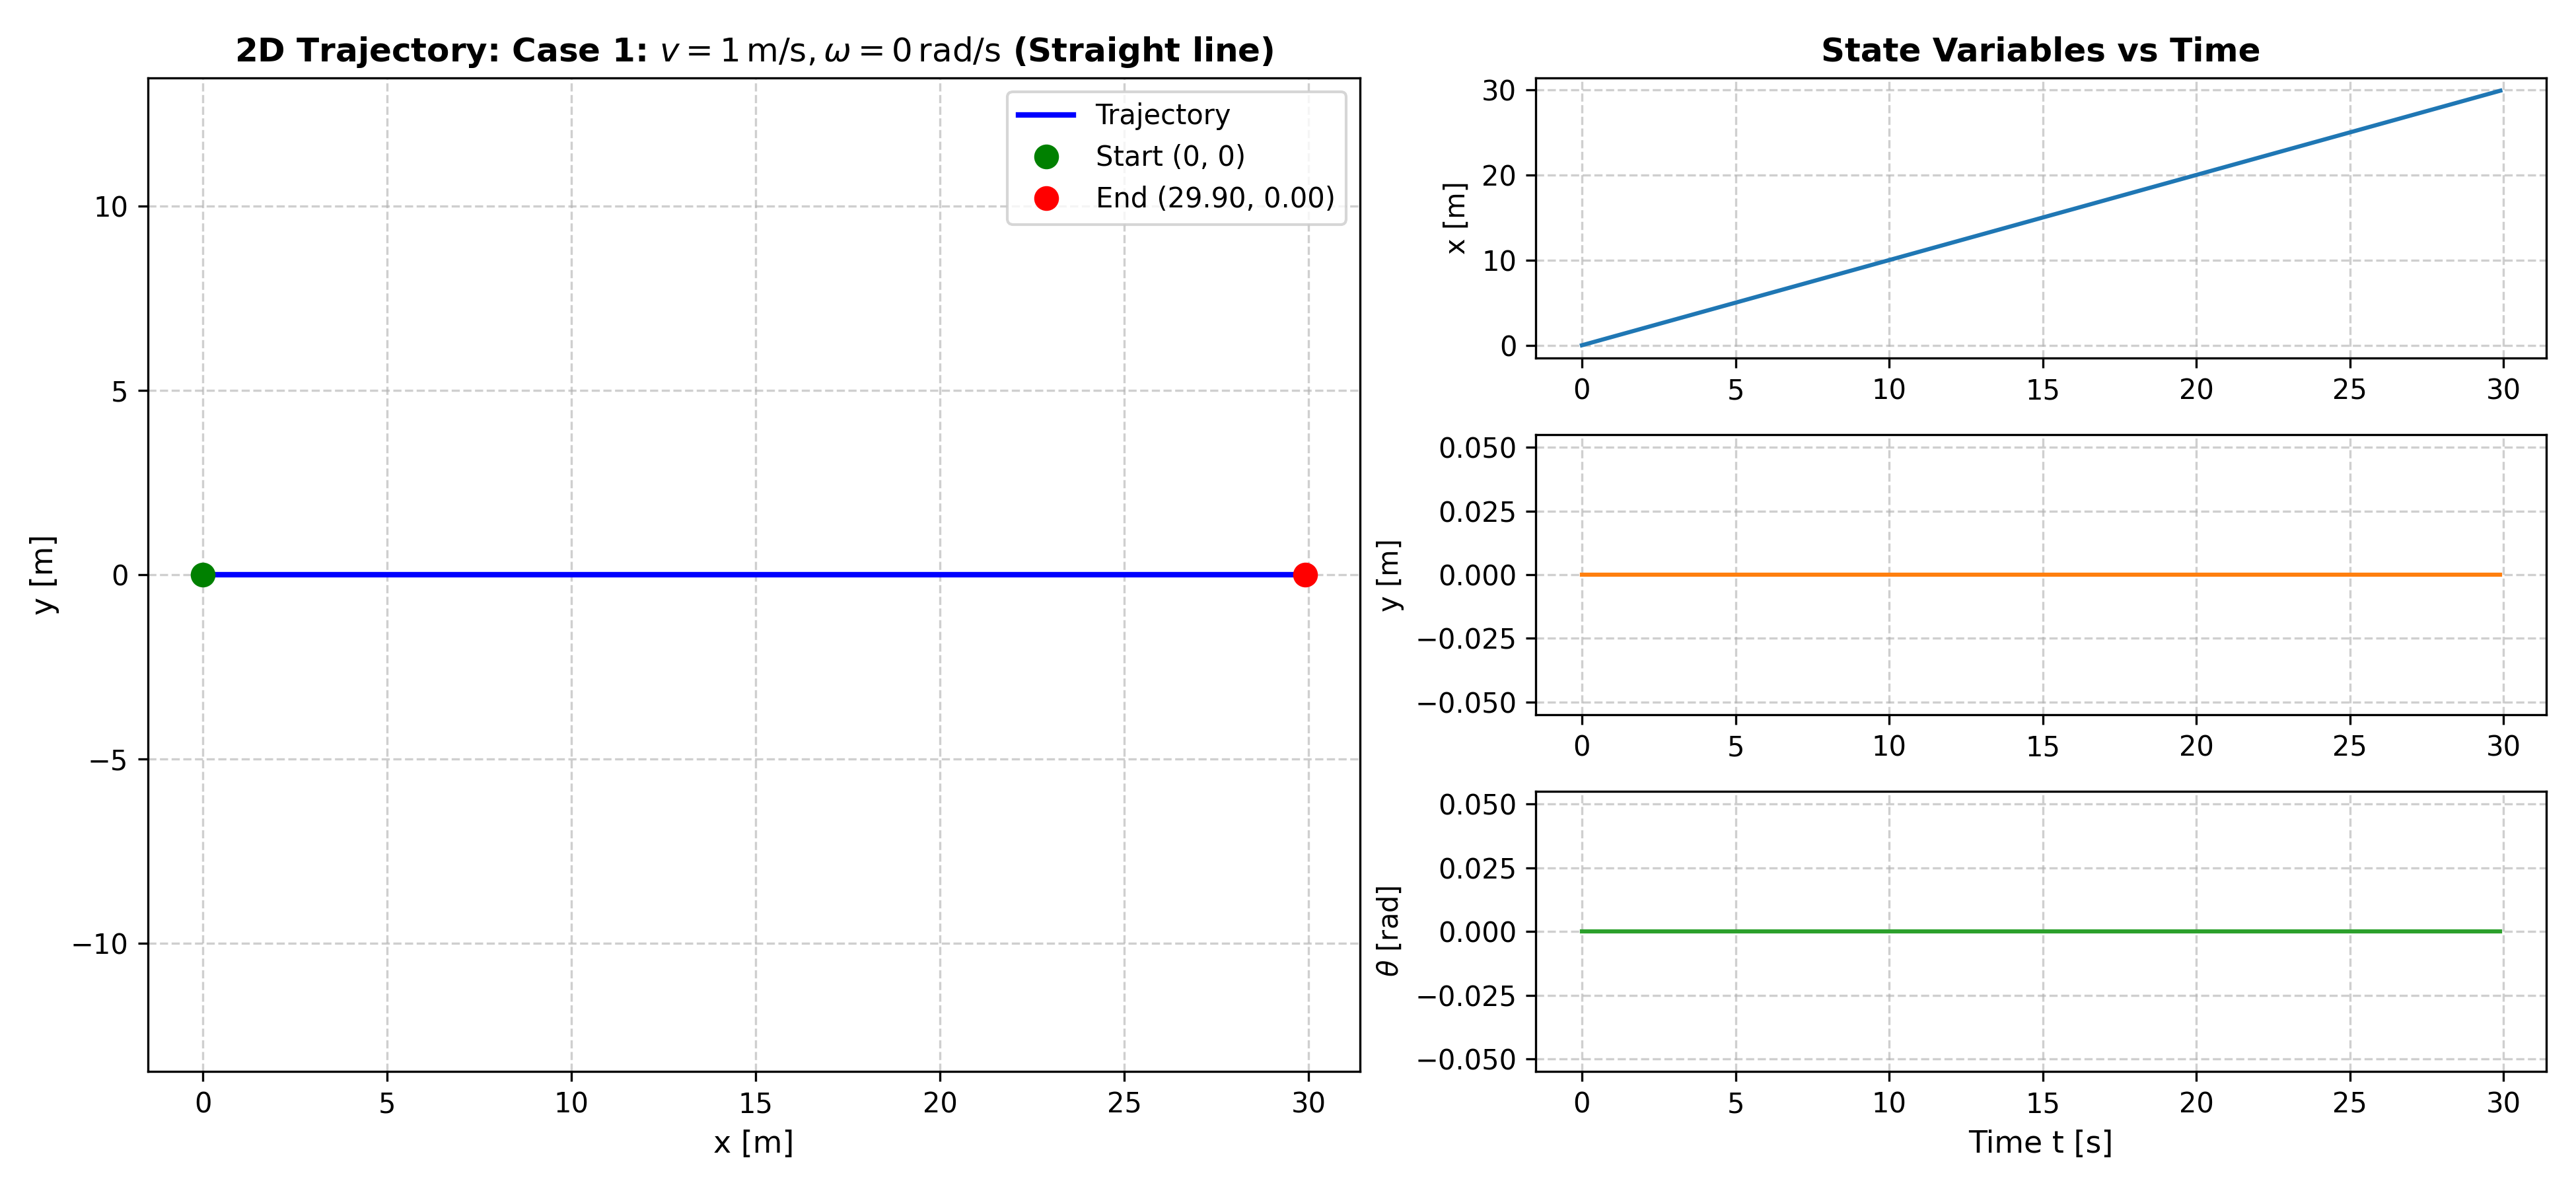
\includegraphics[width=0.78\linewidth]{img/q2_case1.png}
        \captionof{figure}{Trajectory and state variables for Case 1}
    \end{center}
    
    \textbf{Observations:} With zero angular velocity ($\omega = 0$), the robot's heading remains constant at $\theta(t) = 0\,\text{rad}$. The linear velocity drives the robot in a straight line along the global $X$-axis, so we see only x increase, and y and theta remain constant.

    \vspace{1em}
    \paragraph{Case 2: $\begin{bmatrix} v, \omega \end{bmatrix}^\top = \begin{bmatrix} 0, 0.5 \end{bmatrix}^\top$}
    \begin{center}
        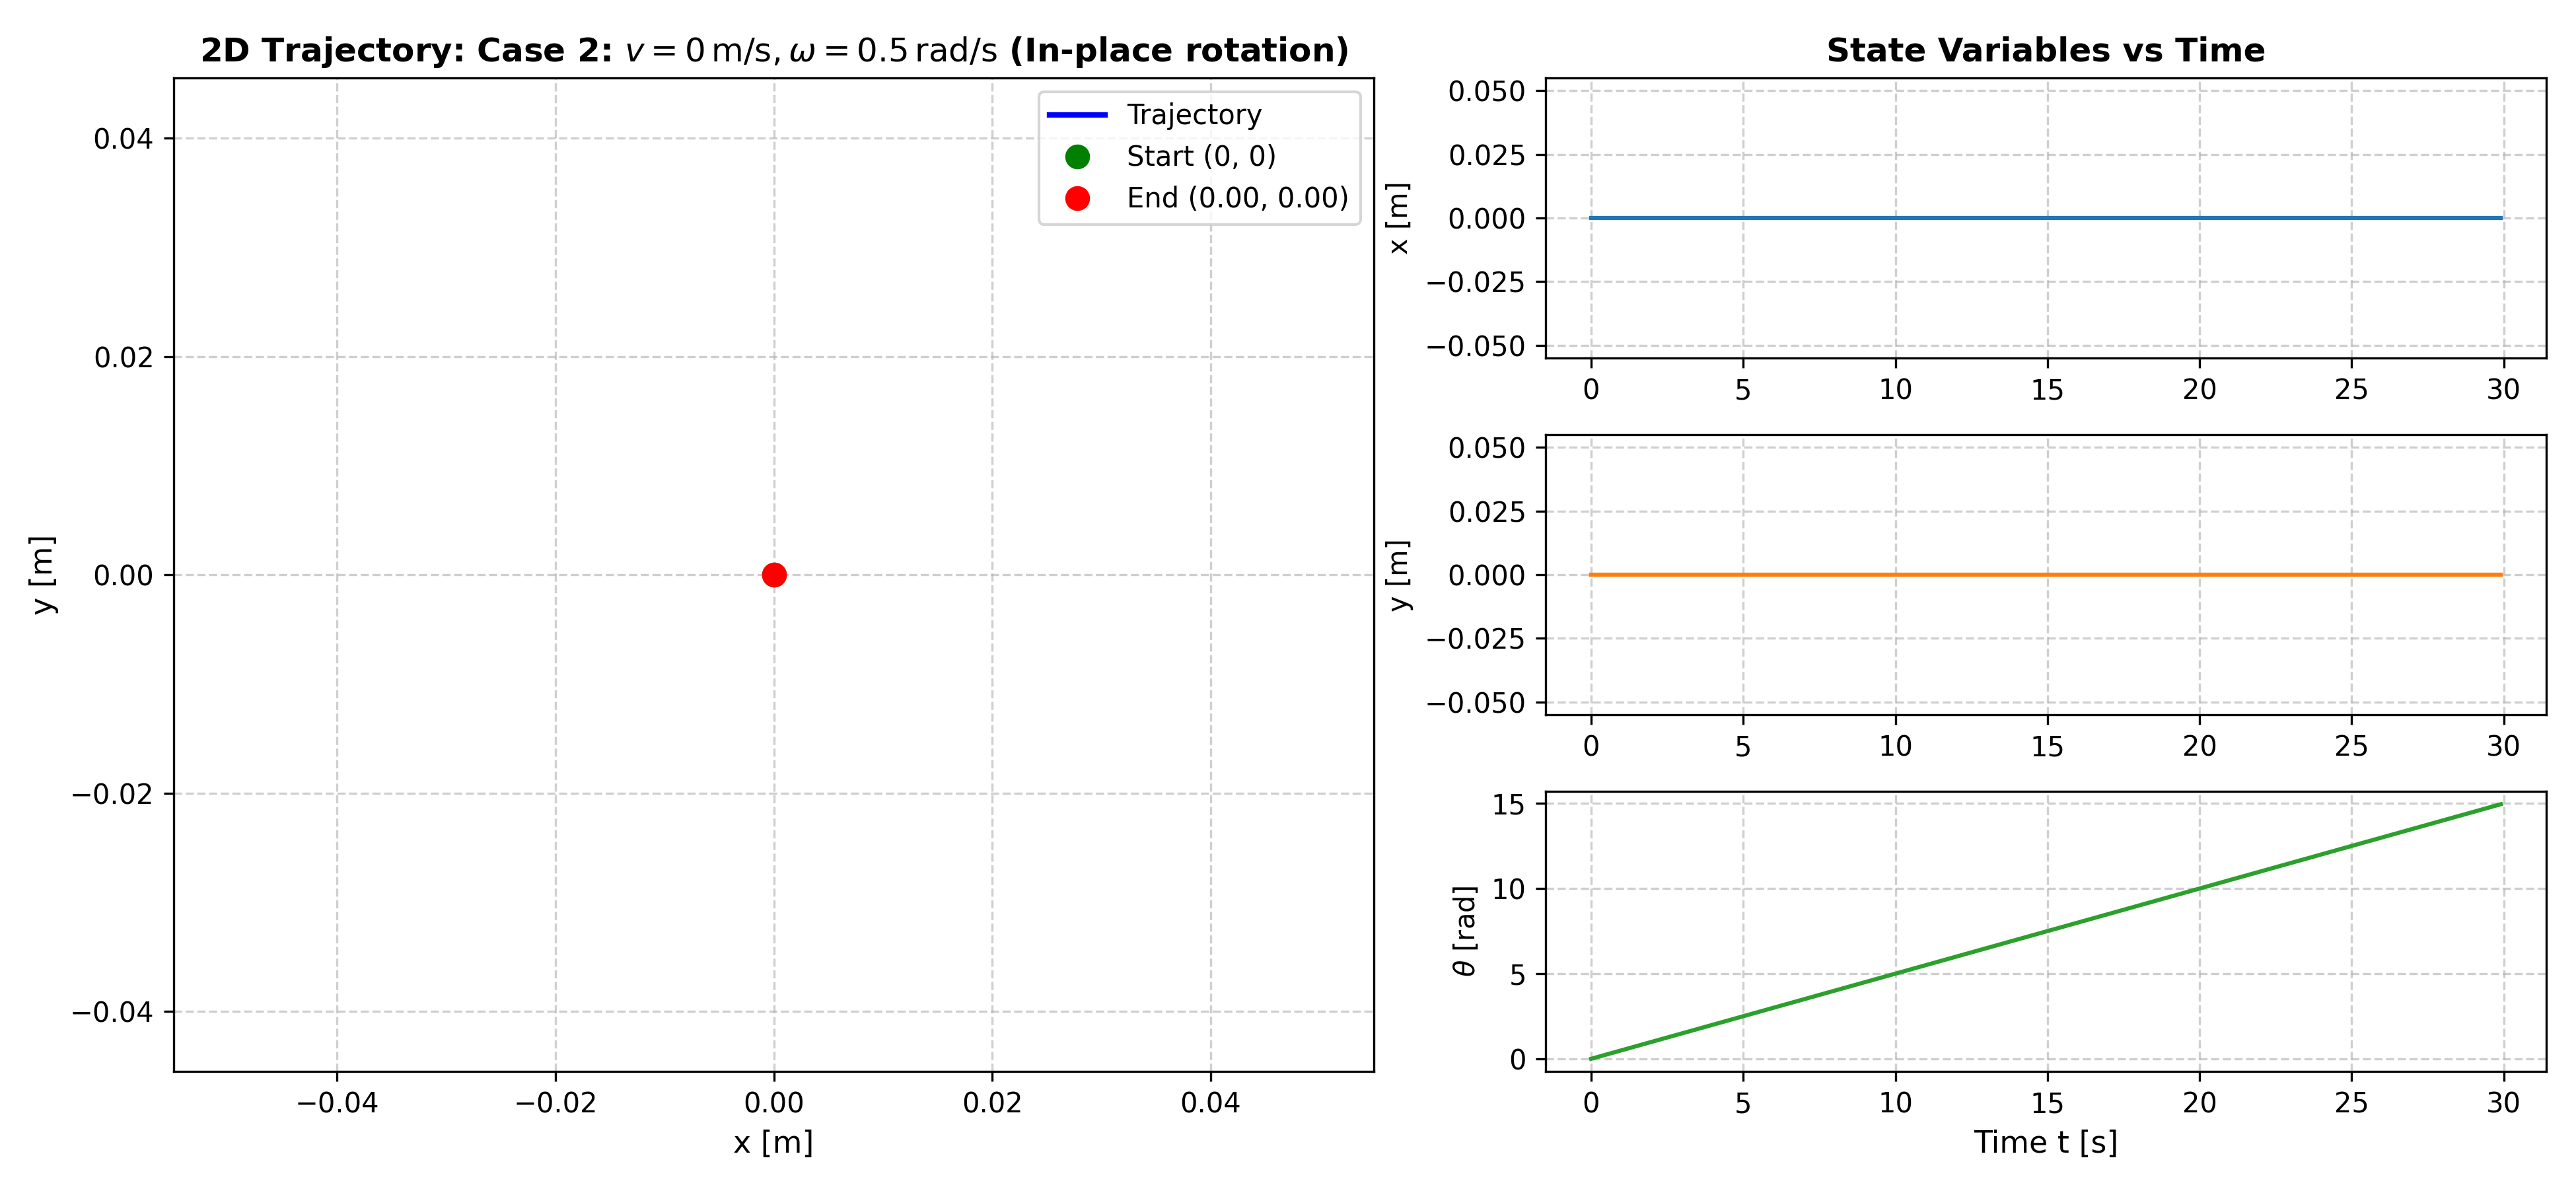
\includegraphics[width=0.85\linewidth]{img/q2_case2.png}
        \captionof{figure}{Trajectory and state variables for Case 2}
    \end{center}
    
    \textbf{Observations:} With zero linear velocity ($v = 0$), there is no translation, and the robot rotates strictly in place about its center. The position coordinates don't change. The heading $\theta(t)$ increases linearly visible only in the $\theta$ plot.

    \vspace{1em}
    \paragraph{Case 3: $\begin{bmatrix} v, \omega \end{bmatrix}^\top = \begin{bmatrix} 1, 0.5 \end{bmatrix}^\top$}
    \begin{center}
        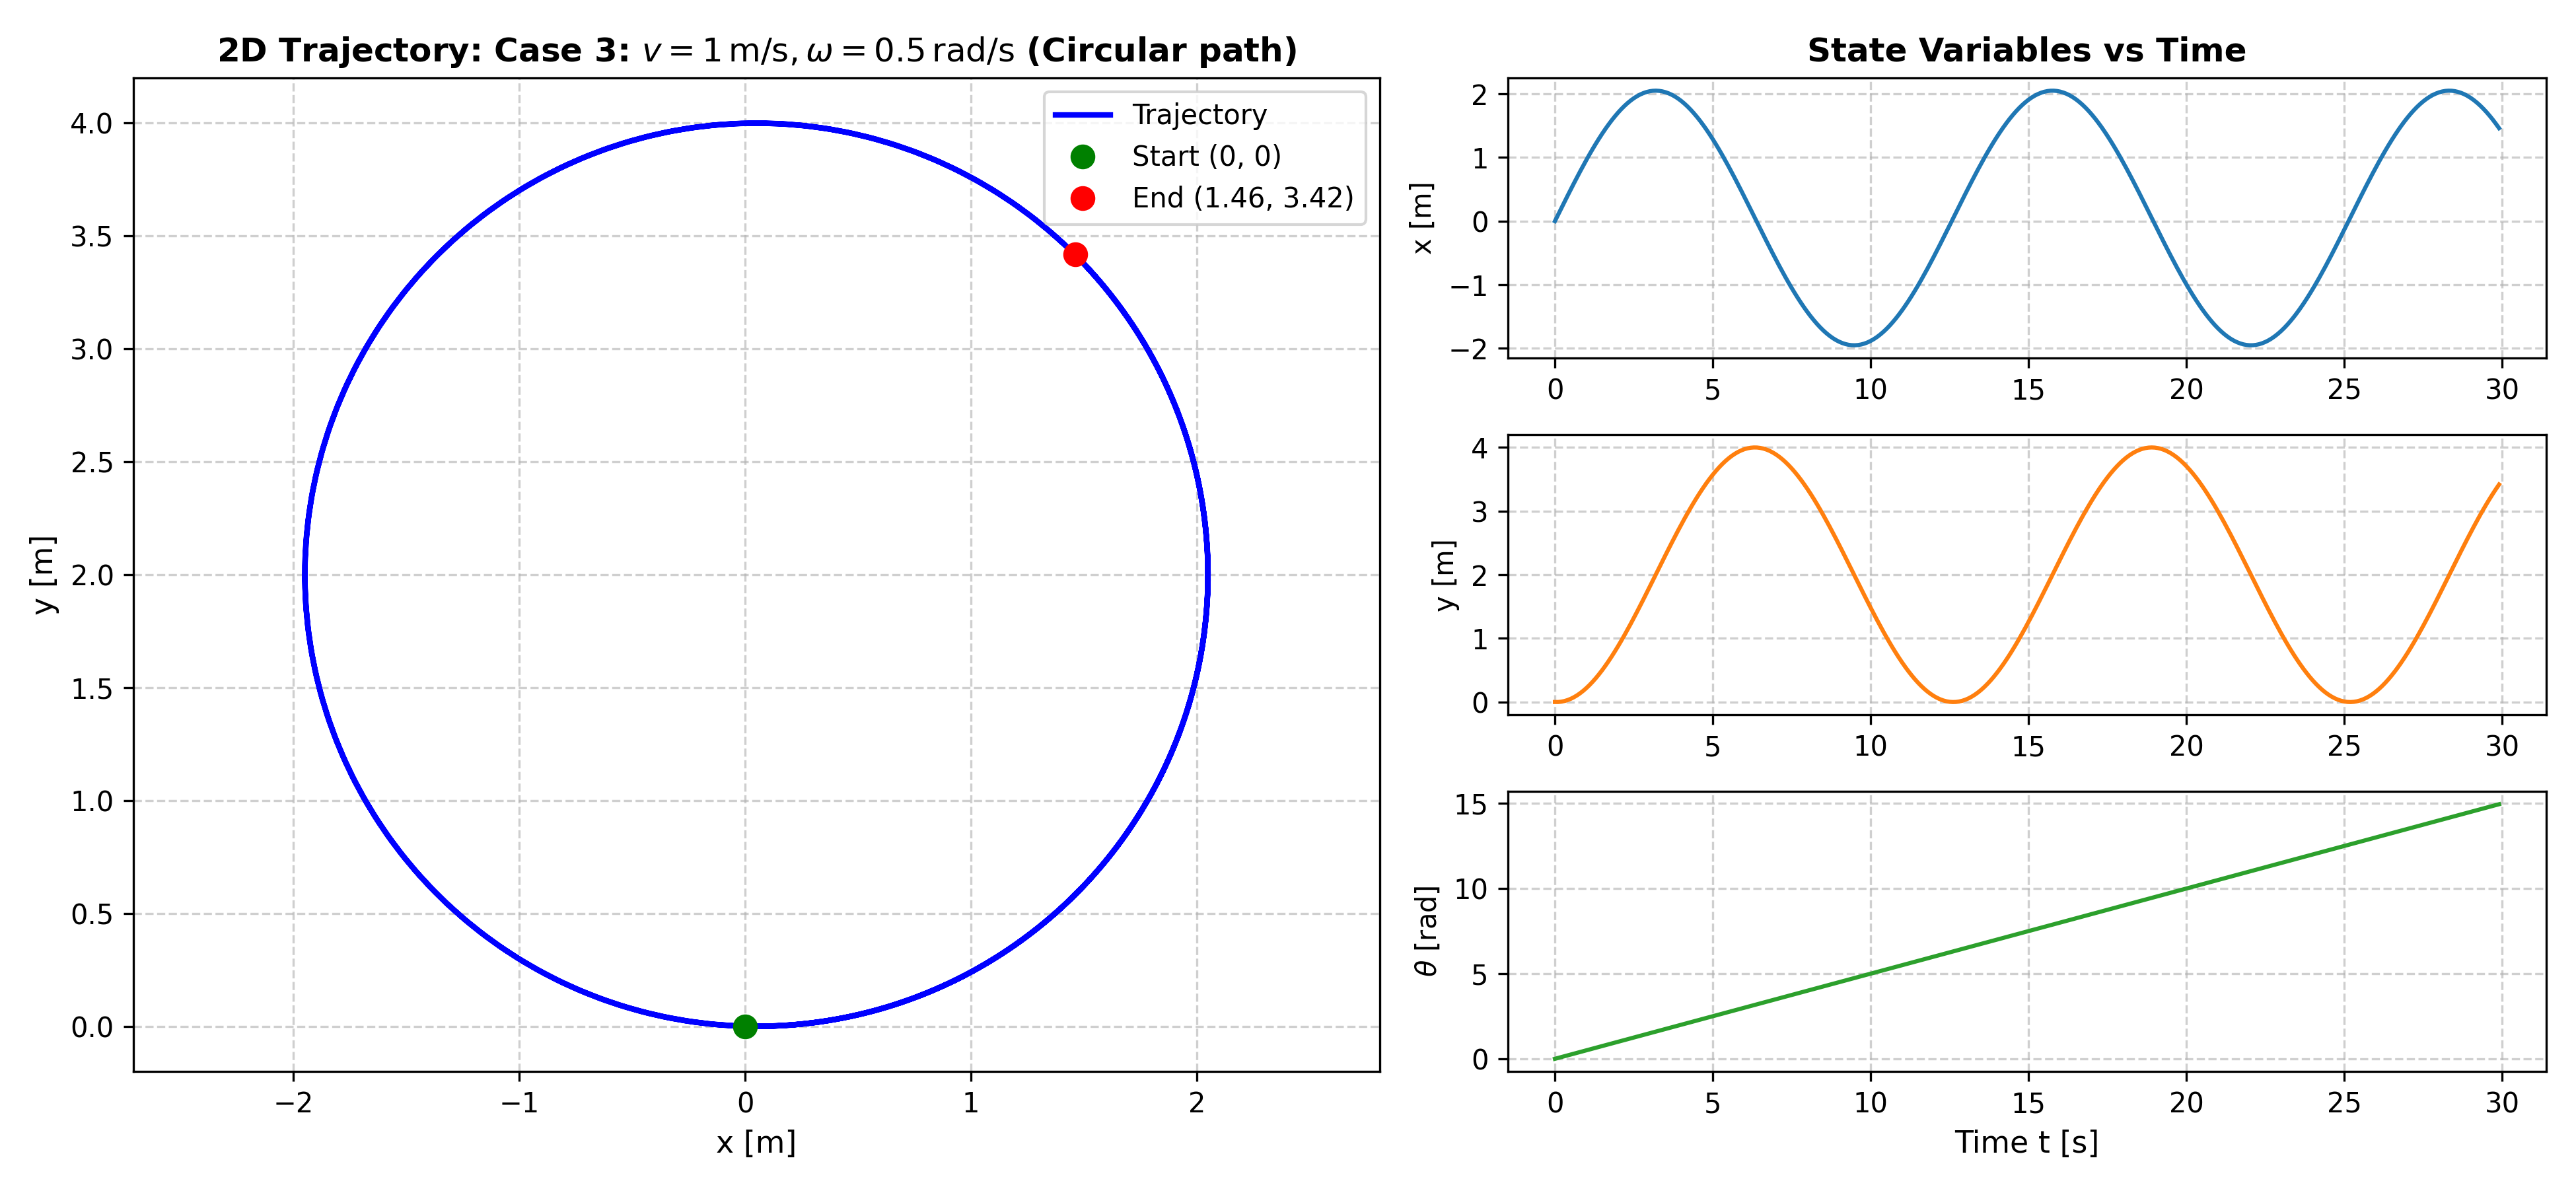
\includegraphics[width=0.85\linewidth]{img/q2_case3.png}
        \captionof{figure}{Trajectory and state variables for Case 3}
    \end{center}
    
    \textbf{Observations:} Combining constant linear and angular velocities yields a circle.
    Particularly the ratio of linear velocity to anglular velocity is defines the radius of the circle as $R = \frac{v}{\omega} = \frac{1}{0.5} = 2\,\text{m}$.
    We can visually confirm the robot traces a circle of radius $2\,\text{m}$ centered at $(0, 2)\,\text{m}$. 
    The position states $x(t)$ and $y(t)$ oscillate sinusoidally with an amplitude of $2\,\text{m}$
    which is a neat corelation to notice since indeed as we trace around a circle we expect the x and y components to form cos and sin respectively.

    \vspace{1em}
    \subsubsection*{ii. Velocity Profiles}
    \textbf{Profile:} $\begin{bmatrix} v(t) \\ \omega(t) \end{bmatrix} = \begin{bmatrix} 1 + 0.2\sin(t) \\ 0.2 + 0.6\cos(t) \end{bmatrix}$
    
    \begin{center}
        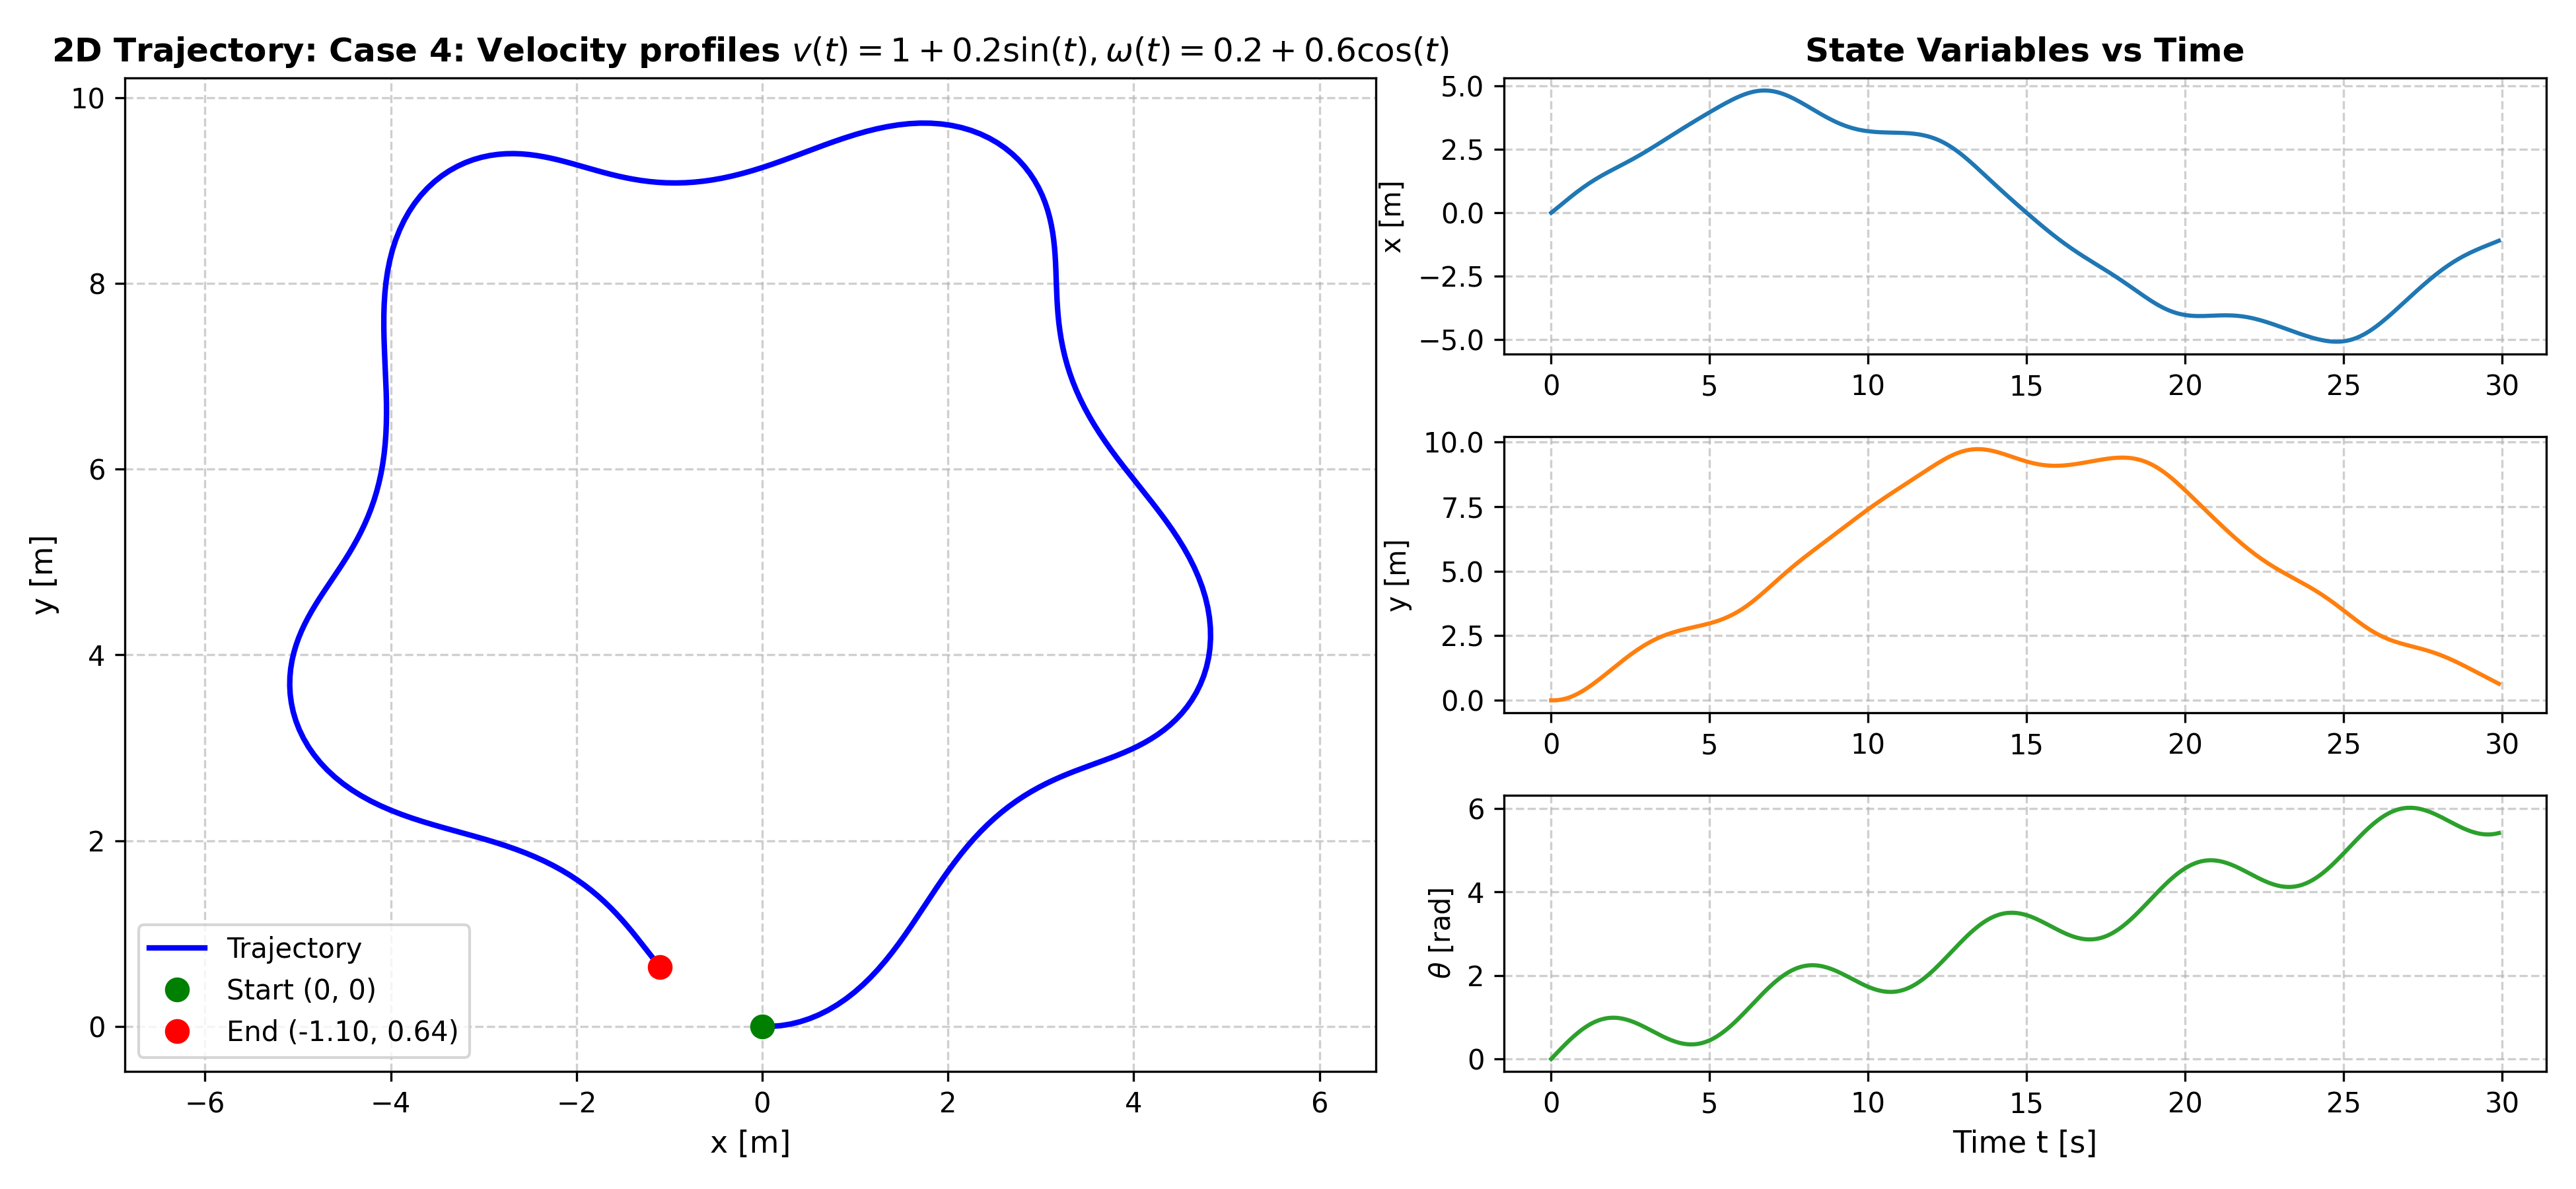
\includegraphics[width=0.85\linewidth]{img/q2_case4.png}
        \captionof{figure}{Trajectory and state variables for Case 4.}
    \end{center}
    
    \textbf{Observations:} The angular rate $\omega(t)$ has a bias/offset of $0.2\,\text{rad/s}$, so it produces an overall net counter-clockwise trajectory while the $0.6\cos(t)$ component periodically wiggles the curvature. Coupled with the oscillating speed $v(t)$, the robot traces an undulating, complex, yet periodic trajectory.

    \item Given robot parameters $T = 0.3\,\text{m}$ (track width) and $r = 0.15\,\text{m}$ (wheel radius).

    The linear velocities at the left and right wheels are:
    \begin{align}
        v_L^w &= \omega\left(R - \frac{T}{2}\right) = v - \frac{T\omega}{2} \\
        v_R^w &= \omega\left(R + \frac{T}{2}\right) = v + \frac{T\omega}{2}
    \end{align}

    The corresponding wheel speeds $u_r(v, \omega)$ and $u_l(v, \omega)$ (in rad/s) are:
    \begin{align}
        u_r(v, \omega) &= \frac{1}{r} v_R^w = \frac{1}{r}\left(v + \frac{T\omega}{2}\right) = \frac{1}{0.15}(v + 0.15\omega) \label{eq:ur} \\
        u_l(v, \omega) &= \frac{1}{r} v_L^w = \frac{1}{r}\left(v - \frac{T\omega}{2}\right) = \frac{1}{0.15}(v - 0.15\omega) \label{eq:ul}
    \end{align}

    Applying this to the three constant velocity cases:
    \begin{enumerate}[label=\arabic*.]
        \item For $\begin{bmatrix} v, \omega \end{bmatrix}^\top = \begin{bmatrix} 1, 0 \end{bmatrix}^\top$:
        \begin{equation*}
            u_r(v, \omega) = 6.667\,\text{rad/s}, \quad u_l(v, \omega) = 6.667\,\text{rad/s}
        \end{equation*}

        \item For $\begin{bmatrix} v, \omega \end{bmatrix}^\top = \begin{bmatrix} 0, 0.5 \end{bmatrix}^\top$:
        \begin{equation*}
            u_r(v, \omega) = 0.5\,\text{rad/s}, \quad u_l(v, \omega) = -0.5\,\text{rad/s}
        \end{equation*}

        \item For $\begin{bmatrix} v, \omega \end{bmatrix}^\top = \begin{bmatrix} 1, 0.5 \end{bmatrix}^\top$:
        \begin{equation*}
            u_r(v, \omega) = 7.167\,\text{rad/s}, \quad u_l(v, \omega) = 6.167\,\text{rad/s}
        \end{equation*}
    \end{enumerate}

    \paragraph{Simulation Modification for Wheel Speed Inputs:}
    Solving the system of linear equations in \eqref{eq:ur} and \eqref{eq:ul}:
    \begin{equation}
        \omega = r\frac{u_r - u_l}{T}, \quad v = r\frac{u_r + u_l}{2}
    \end{equation}

    Substituting these directly into the equation from earlier:
    \begin{align}
        \dot{p} &= \begin{bmatrix} \dot{x} \\ \dot{y} \\ \dot{\theta} \end{bmatrix} = \begin{bmatrix} \cos\theta & 0 \\ \sin\theta & 0 \\ 0 & 1 \end{bmatrix} \begin{bmatrix} v \\ \omega \end{bmatrix} \notag \\
        &= r \begin{bmatrix} \cos\theta & 0 \\ \sin\theta & 0 \\ 0 & 1 \end{bmatrix} \begin{bmatrix} \frac{1}{2}(u_r + u_l) \\ \frac{1}{T}(u_r - u_l) \end{bmatrix} \notag \\
        &= r \begin{bmatrix} \frac{1}{2}\cos\theta\,(u_r + u_l) \\ \frac{1}{2}\sin\theta\,(u_r + u_l) \\ \frac{1}{T}(u_r - u_l) \end{bmatrix} \notag \\
        &= r \begin{bmatrix} \frac{1}{2}\cos\theta & \frac{1}{2}\cos\theta \\ \frac{1}{2}\sin\theta & \frac{1}{2}\sin\theta \\ \frac{1}{T} & -\frac{1}{T} \end{bmatrix} \begin{bmatrix} u_r \\ u_l \end{bmatrix}
    \end{align}
    This matrix expression for $\dot{p}$ in terms of $[u_r, u_l]^\top$ now substitutes in exactly where $\dot{p}$ was computed previously in the Forward Euler update loop ($p_{\text{new}} = p_{\text{old}} + \dot{p}\,\Delta t$).
\end{enumerate}

